\documentclass[11pt]{article}

\usepackage{amsmath}
\usepackage{amsfonts} 
\usepackage{amsthm}
\usepackage{blkarray}
\usepackage{caption}
\usepackage{enumitem} 
\usepackage{mathtools}
\usepackage{tikz}
\usepackage[top=1.5cm,bottom=2cm,left=1.25cm,right=1.75cm,marginparwidth=1.75cm]{geometry}
\setlength{\parindent}{0cm}

\newcommand{\n}{\vspace{0.2cm}}

\usetikzlibrary{decorations.pathreplacing,decorations.markings}

\tikzset{unode/.style = {
    circle, 
    draw=black,
    fill=white,
    inner sep=1.5pt,
    minimum size=1.5pt }}
\tikzset{uedge/.style = {
    draw=black }}

\def\lc{\left\lceil}   
\def\rc{\right\rceil}
\def\lf{\left\lfloor}   
\def\rf{\right\rfloor}
\def\N{\mathbb N}

\newtheorem{theorem}{Theorem}

\title{\vspace{-1.0cm}MATH 5707 Final}
\author{Fletcher Gornick}
\date{April 28, 2023}

\begin{document}
\maketitle
  \begin{enumerate}
    \item (20 points) \textbf{True or False}.  To receive full credit, assertions which are true must be proven, and those that are false must have a counterexample exhibited.
      \begin{enumerate}
        \item (5 points) If a graph \(G\) has degree sequences \((2,2,4,4,4,4,4)\) then it is eulerian, that is, it contains a (closed) Euler tour. \n\\
          \textbf{FALSE}.  \(G\) could still be disconnected.  The following graph has the above degree sequence but clearly contains no euler tour.
          \begin{center}
            \resizebox{!}{4cm} {
              \begin{tikzpicture}[every node/.style={circle,draw}, every loop/.style={in=150,out=210}]
                \node (1) at (0,3) {};
                \node (2) at (4,3) {};
                \node (3) at (10,6) {};
                \node (4) at (13.5,3.5) {};
                \node (5) at (12,0) {};
                \node (6) at (8,0) {};
                \node (7) at (6.5,3.5) {};

                \draw (1) edge [bend right] (2);
                \draw (1) edge [bend left] (2);

                \draw (3) edge [bend right] (4);
                \draw (3) edge [bend left] (4);
                \draw (4) edge [bend right] (5);
                \draw (4) edge [bend left] (5);
                \draw (5) edge [bend right] (6);
                \draw (5) edge [bend left] (6);
                \draw (6) edge [bend right] (7);
                \draw (6) edge [bend left] (7);
                \draw (7) edge [bend right] (3);
                \draw (7) edge [bend left] (3);
              \end{tikzpicture}
            }
          \end{center}

        \item (5 points) If a tree has \(n\) vertices in total, in which \(\ell\) of them are leaves and all other vertices have degree 3, then \(\ell = \frac{n+2}2\). \n\\
          \textbf{TRUE}.  We can first note that, theorem 1.1 of the textbook states \(2\varepsilon = \sum_{v \in V} d_G(v)\), and theorem 2.2 states \(\varepsilon = \nu-1\).  With this we get the following equalities,
          \begin{align*}
            2(n-1) &= 2 \varepsilon \\
                   &= \sum_{v \in V} d_G(v) \\
                   &= \sum_{\text{leaves }} d_G(v) + \sum_{\text{non-leaves}} d_G(v) \\
                   &= \ell \cdot 1 + (n - \ell) \cdot 3 \\
                   &= 3n - 2\ell.
          \end{align*}

          Finally, rearranging \(2(n-1) = 3n-2\ell\), we see \(\ell = \frac{3n - 2(n-1)}{2} = \frac{n+2}{2}\). \n

        \item (5 points) Given a graph \(G\) with connected components \(G_1,G_2,\hdots,G_r\), it's chromatic polynomial \(p_G(k)\) always satisfies
          \[p_G(k) = p_{G_1}(k) \cdot p_{G_2}(k) \cdot \cdots \cdot p_{G_r}(k)\]
          \textbf{TRUE}.  Since each connected component shares no edges with another, the coloring of one connected component has no effect on the coloring of another.  So \(p_{G_i \sqcup G_j}(k) = p_{G_i}(k) \cdot p_{G_j}(k)\).  Repeating for multiple graphs gives the above inequality. \n

        \item (5 points) Recall (from lecture or Bondy \& Murty’s Section 3.2) that for every graph \(G\), one can uniquely define 2-connected subgraphs \(B_1,B_2,\hdots,B_s\) called it's \textit{blocks} or \textit{2-connected components}, whose union is \(G\).  Assuming \(G\) is connected, then it's chromatic polynomial always satisfies
          \[p_G(k) = \frac{p_{B_1}(k) \cdot p_{B_2}(k) \cdot \cdots \cdot p_{B_s}(k)}{k^{s-1}}.\]
          \textbf{TRUE}.  If we simply look at the first block \(B_1\), we know it'll have \(p_{B_1}(k)\) possible \(k\)-colorings.  Now \(B_1\) should share a vertex with at least one other block, suppose our blocks are ordered in a way such that \(V(B_i) \cap V(B_j) \neq \emptyset \text{ when } j = i+1\).  So \(B_1\) shares some vetex \(u\) with \(B_2\).  For each \(k\)-coloring of \(B_1\), \(u\) must be fixed in any coloring of \(B_2\) in order to not conflict.  We've now reduced the number of possible colorings for \(B_2\) by a factor of \(k\), since it's vertex \(u\) is fixed. \n

           Now we move on to block \(B_3\) sharing vertex \(v\) with \(B_2\).  Again \(B_3\) will have \(\frac{p_{B_3}(k)}{k}\) colorings because \(v\) must be fixed.  We also know that \(B_3\) cannot share a vertex with \(B_1\), because if it did then we'd know \(B_1 \cup B_i \cup B_j\) would form a new 2-connected component which wouldn't make sense. \n

          We can continue coloring all our blocks like this until reaching the last block \(B_s\) noting that \(B_2, \hdots, B_s\) have a factor of \(k\) fewer vertex independent colorings.  Again, \(B_s\) can only share one vertex with any other set, another would lead to the whole graph being 2-connected.  So we conclude
          \[p_G(k) = \frac{p_{B_1}(k) \cdot p_{B_2}(k) \cdot \cdots \cdot p_{B_s}(k)}{k^{s-1}}.\]
      \end{enumerate} \n

    \item (20 points) Define for each \(n=1,2,3,\hdots\) a simple bipartite graph \(G_n = (X \sqcup Y, E)\) with vertex set \(V = X \sqcup Y\) partitioned into two sets of sice \(n\) labeled
      \begin{align*}
        X &= \{x_1, \hdots, x_n\}, \\
        Y &= \{y_1, \hdots, y_n\},
      \end{align*}
      and edge set \(E\) of size \(n^2 - n\) defined as follows:
      \[E := \{x_iy_j \mid 1 \leq i,j \leq n, \; i \neq j\}.\]
      \begin{enumerate}
        \item (10 points) For exactly which values of \(n=1,2,3,\hdots\) is \(G_n\) eulerian? \n\\
          Only for odd \(n \geq 3\).  When \(n\) even, every vertex must be connected to \(n-1\) other vertices, meaning that all the degrees are odd.  By similar reasoning, all vertices have even degree for odd \(n\), and all graphs \(G_n\) are clearly connected for \(n \geq 3\), so the result follows immediately from theorem 4.1. \n

        \item (10 points) For exactly which values of \(n=1,2,3,\hdots\) is \(G_n\) hamiltonian? \n\\
          All graphs \(G_n\) with \(n \geq 3\) are hamiltonian.  For odd \(n\), we can construct a Hamilton cycle like so 
          \[E(C) := \{x_iy_j \mid 0 \leq i,j < n, \; i-j \equiv \pm 1 \pmod n\}\]
          So we get \(x_0 \to y_1 \to x_2 \to \cdots \to x_{n-1} \to y_0 \to x_1 \to \cdots \to x_{n-2} \to y_{n-1} \to x_0\). \n

          For even \(n \geq 4\), I don't know how to easily express the Hamilton cycle, but there will always be one of this form:
          \[x_0 \to y_1 \to x_2 \to \cdots \to y_{n-1} \to x_1 \to y_0 \to x_{n-1} \to y_{n-2} \to x_{n-3} \to \cdots \to x_3 \to y_2 \to x_0.\]
      \end{enumerate}

    \item (20 points) Let \(G = (V,E)\) be a simple graph with maximum vertex degree \(\Delta(G)\), and maximum size of a \textit{stable} subset \(\alpha(G)\).  Prove that
      \[\alpha(G) \geq \frac{\nu}{1 + \Delta(G)}.\]
      \begin{proof}
        Suppose to the contrary, \(\alpha(1 + \Delta) < \nu\), and let \(V'\) be a maximum-sized stable set of vertices in \(G\) (with \(|V'| = \alpha(G)\)). \n

        Each vertex \(v \in V'\) has at most \(\Delta\) neighbors, so if we gather each \(v \in V'\) along with all of \(v\)'s neighbors, we get no more than \(\sum_{v \in V'} (1+d(v))\) vertices (probably less unless all \(v \in V'\) have no adjacent vertices in common). This gives us
        \[\#\{\text{vertices reachable from } V'\} \leq \sum_{v \in V'} (1+d(v)) \leq \sum_{v \in V'} (1+\Delta) = \alpha(1+\Delta) < \nu,\]
        But this means that there exists a vertex \(u \in V \setminus V'\) that isn't adjacent to any \(v \in V'\), meaning that \(V'\) cannot be a maximum stable set, which is a contradiction.
      \end{proof}
      

    \item (20 points) When a soccer-ball-like sphere is made up only of pentagonal and hexagonal faces, sewn together so that its seams form a graph which is 3-regular (at every vertex, there are exactly 3 edges incident), how many pentagonal faces will there be in total?

(Note: it turns out that the number of hexagons can vary, but you will end up proving that the number of pentagonal faces is a fixed number!) \n\\
From lecture, we know that there are only four regular polyhedrons, one of which being the dodecahedron with degree-5 faces and degree-3 vertices.  The dodecahedron has 12 faces, and we can represent it on the plane like so (unbounded face on outside):
      \begin{center}
        \resizebox{!}{8cm} {
          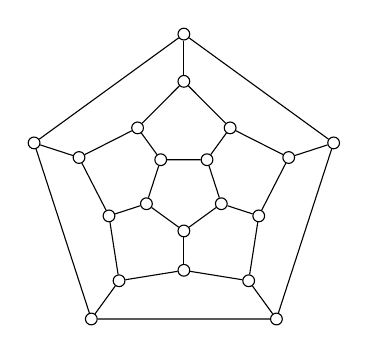
\begin{tikzpicture}[every node/.style={circle,draw}, every loop/.style={in=150,out=210}]
            \foreach \x in {0,1,2,3,4}{
                \node[unode] (o\x) at (18+\x*72:2cm) {};
                \node[unode] (i\x) at (18+\x*72:1.4cm) {};
                \node[unode] (ii\x) at (54+\x*72:1cm) {};
                \node[unode] (iii\x) at (54+\x*72:0.5cm) {};
            }
            \foreach \x in {0,1,2,3,4}{
                \path[uedge] (o\x) edge (i\x); 
                \path[uedge] (ii\x) edge (iii\x);
            }
            \path[uedge] (o0)--(o1)--(o2)--(o3)--(o4)--(o0);
            \path[uedge] (iii0)--(iii1)--(iii2)--(iii3)--(iii4)--(iii0);
            \path[uedge] (i0)--(ii0)--(i1)--(ii1)--(i2)--(ii2)--(i3)--(ii3)--(i4)--(ii4)--(i0);
                  \end{tikzpicture}
                }
      \end{center}
      Since planar graphs are also embeddable on spheres, we can visualize this by just shrinking the unbounded face and thinking of it as the other side of the soccer ball, or you could simply think of a rounded dodecahedron.  Also note that splitting any vertex into 3, repeating the 3 edges for each of the two added vertices, will keep 12 pentagons and it'll stay 3 regular, but there's now an extra hexagon.  Doing this on all vertices once will result in the soccer ball we're familiar with. \n

      Now we show that there are always 12 pentagonal faces.
      \begin{proof}
        Let \(F\) denote the set of faces in \(G\), and \(f = |F|\).  Also let \(f_5 := |\{f \in F \mid d_G(f) = 5\}|\) be the number of pentagonal faces, and \(f_6 := |\{f \in F \mid d_G(f) = 6\}|\) be the number of hexagonal faces.  Applying theorem 1.1 and theorem 9.4, we see that
        \[3\nu = \sum_{v \in V}d_G(v) = 2\varepsilon = \sum_{v \in F} d_G(f) = 5f_5 + 6f_6,\]
        We can now use this result to rewrite Euler's formula in terms of both \(\nu\) and \(f = f_5+f_6\).
        \begin{align}
          -\frac12\nu + f_5 + f_6 &&=&& \nu - \frac32\nu + f_5 + f_6 &&=&& \nu - \varepsilon + f &&=&& 2 \\
          \nu - \frac32f_5 - 2f_6 &&=&& \nu - \frac52f_5 - 3f_6 + f_5 + f_6 &&=&& \nu - \varepsilon + f &&=&& 2
        \end{align}
        Finally if we add \(2 \cdot (1)\) onto \((2)\), we get \(\frac12f_5 = 6 \implies f_5 = 12\).
      \end{proof}
      


    \item (20 points)
      \begin{enumerate}
        \item (10 points) Show that in any directed graph \(D = (V,A)\), one has
          \[\sum_{v \in V} d_D^+(v) = \sum_{v \in V} d_D^-(v),\]
          where \(d_D^-(v), d_D^+(v)\) are the \textit{indegree} and \textit{outdegree} of vertex \(v\).
          \begin{proof}
            The outdegree of a vertex is the number of times an edge leaves it, so \(\sum_{v \in V} d_G^+(v)\) counts the number of times an edge leaves a vertex.  Since every directed edge that leaves a vertex must also enter a vertex we have that this sum must also match the number of times an edge enters a vertex, which is exactly \(\sum_{v \in V} d_G^-(v)\).
          \end{proof} \n

        \item (10 points) Let \(G = (V,E)\) be a connected undirected graph with \(|E|\) even.  Show that there exists at least one choice of a directed graph  \(D = (V,A)\) obtained from \(G\) by orienting each edge \(e = xy \in E\) either as the arc \(x \rightarrow y\) or \(x \leftarrow y \in A\), such that \(d_D^+(v)\) is even for all \(v \in V\).
          \begin{proof}
            We induct on the number of vertices.  If \(\nu = 1\), then \(G\) has an even number of loops, so \(d_G^+(v) = \varepsilon\) which is even.  If \(\nu = 2\), then let \(u\) and \(v\) be the two vertices.  We show that all cases of a two-vertex connected graph with an even number of edges has a valid directed orientation fulfilling our claim. \n

            If \(u\) and \(v\) both have an even number of loops and an even number of \(uv\) edges, just orient all the \(uv\) edges in one direction.  If \(u\) has an even number of loops, \(v\) odd, and odd \(uv\) edges, then orient all \(uv\) edges like \(v \to u\), similarly for the case where \(u\) odd and \(v\) even.  Finally if both vertices have an odd number of loops and even number of \(uv\) edges, then orient all but 1 \(uv\) edge in one direction, and the last in the other (we know there are at least two because \(G\) is connected). \n

            Now, suppose for any graph with \(k \geq 2\) vertices and an even number of edges, there exists an orientation of edges such that each vertex has an even outdegree, we show this must also be the case for a graph \(G\) with \(k+1\) vertices. \n

            Since \(G\) is connected with 3+ vertices, there must exist a non-cut vertex \(v\) by corollary 2.7.  So there exists \(v \in V\) such that \(G \setminus v\) still connected. \n

            If \(d_G(v)\) even, then we can take the orientation for \(G \setminus v\) from our inductive hypothesis and add \(v\) back with all the edges leaving \(v\) to construct a correct orientation for \(G\). \n

            If \(d_G(v)\) odd, then take some edge \(v'\) adjacent to \(v\) and give it a loop in \(G \setminus v\) so we have an even number of edges again.  Now find an orientation through the inductive hypothesis and remove the loop.  Adding \(v\) back, make \(v' \to v\) and \(v \to u\) for all other edges. \n

            Therefore, via induction, we've shown that all connected graphs with \(\varepsilon\) even have a directed orientation such that all vertices have an even outdegree.
          \end{proof}
          
      \end{enumerate}
  \end{enumerate}
\end{document}
